\subsubsection{ZCS}
\index{ZCS}
ZCS is a \emph{zeroth level classifier system} originally proposed in \cite{WilsonZCS}.
ZCS preserves most of the functionality of traditional LCS's, but it is a very simplified version, which aids in the understanding of the classifier and its actions.
This was a very useful contribution, because many of the problems with LCS's before then were their overly complex and detailed nature.
A good short summary of ZCS can be found in
\cite{EibenSmith}, and this summary is based primarily on that.
The basic structure of ZCS is graphically illustrated in Figure~\ref{fig:zcs}.

In ZCS there is no message list, a much-welcomed simplification of the traditional LCS.
This comes with a cost: there is no explicit method for transmitting information between cycles without the message list.
This makes the interface entirely dependent on the interface of the system with its environment, and thus assumes a Markov process.
This is most definitely an invalid assumption for real-world traded markets and for other time-series data.

\begin{figure}
\begin{center}
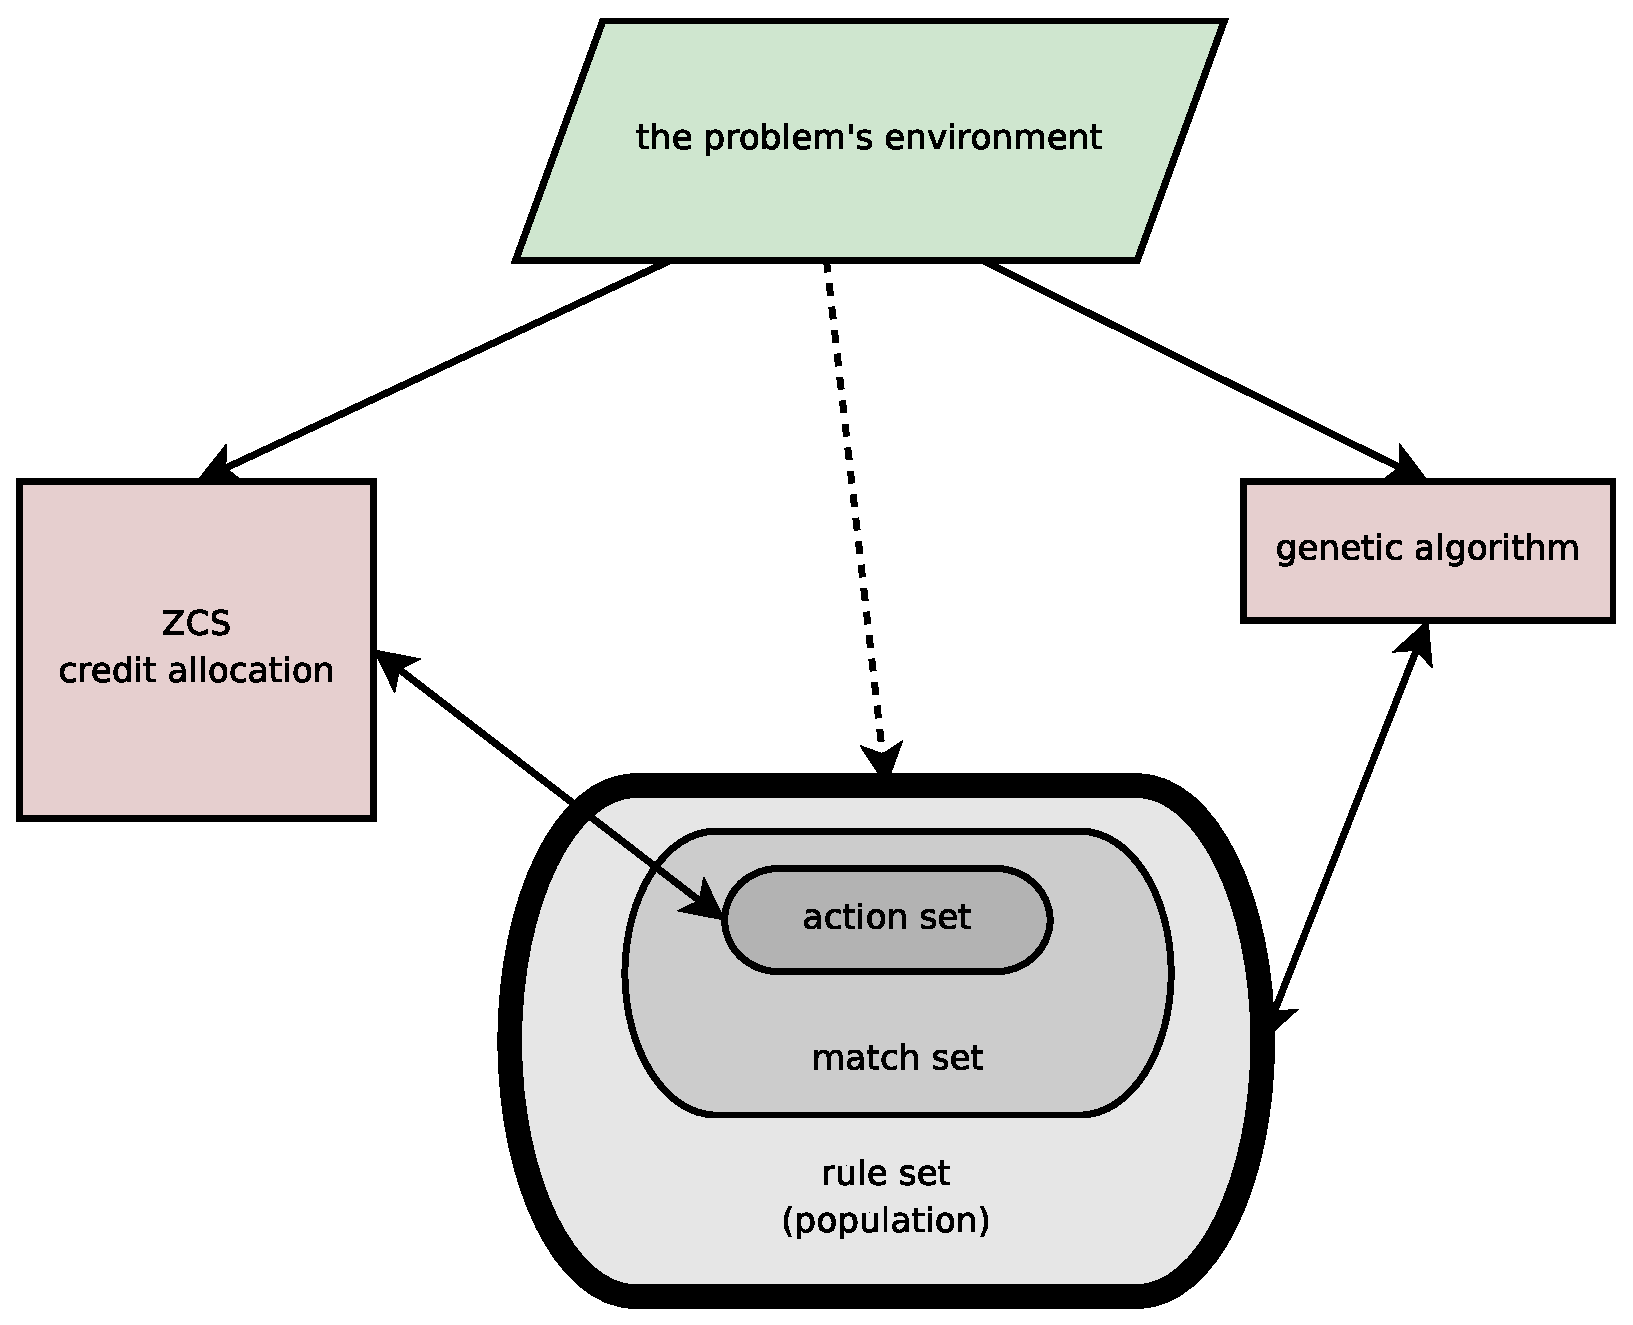
\includegraphics[width=4in]{zcs-basic-diagram.eps}
\caption{ZCS's basic structure}
\label{fig:zcs}
\end{center}
\end{figure}

Each rule $r$ is of the form $r = (c, a, s)$ where:
\begin{itemize}
\item
$c$ is the condition matched by the rule $r$ and is comprised of elements from some alphabet, typically $\{0, 1, \#\}$,
where \# is the matching symbol, matching both 0 and 1;
\item
$a$ is the action that the rule $r$ recommends;
\item
and $s$ is the real-valued strength measurement of the rule $r$, $s \in \mathbb{R}$, which determines how much of a vote rule $r$ has in selecting the action to pursue.
\end{itemize}

In each time cycle $t$ the match set $M_t$ is found, a subset of the population,
$M_t \subseteq P$,
with $P$ being the entire population of rules, the rule set.
\index{population}
\index{P@$P$|see{population}}
The members at time cycle $t$ of the match set $M_t$ can be divided into disjoint subsets based on the action they recommend.
With a finite set of possible actions
\begin{equation}
\mathpzc{A} = \{a_0, a_1, \ldots, a_{|\mathpzc{A}|}\}
\end{equation}
and $\mathpzc{A'} \subseteq \mathpzc{A}$ where
\begin{equation}
\mathpzc{A'} = \{a'_0, a'_1, \ldots, a'_{|\mathpzc{A'}|}\}
\end{equation}
comprises all of the actions represented in the match set $M_t$.
For any specific action $a'_i$ represented in the match set $M_t$ we can form the set of all members of the match set that recommend action $a'_i$, represented as
$M_{t,a'_i} \subseteq M_t$ with
\begin{equation}
M_{t,a'_i} = \left\{ r \colon r \in M_t \land a_r = a'_i \right\}.
\end{equation}
The fitness of an action $a'_i \in \mathpzc{A'}$ is then
\begin{equation}
\mathrm{fitness}(a'_i) = \sum_{\forall r \in M_{t,a'_i}} s_r,
\end{equation}
the sum of the fitness of all of the rules $r$ that recommend that particular action present in $M_{t,a'_i}$.
The action to take is selected in a fitness-proportionate method,
choosing the action $a'$ with the greatest fitness.
If $M_t = \emptyset$ then covering must take place;
a random rule that matches the current situation is created by initially setting $c$ to exactly the current situation and then replacing a few elements of $c$ at random with the \# symbol, and that suggests a randomly-selected action.

The credit assignment scheme used by ZCS is somewhat involved, and is referred to as an \emph{implicit bucket brigade}.
It attempts to reward sequences which lead to reward from the environment and which are short.
First, the rules in the population $P$ but excluded from the match set $M_t$ are originally unchanged:
\begin{equation}
s'_r = s_r \forall r \notin M_t.
\end{equation}
Next, the rules in the match set $M_t$ but excluded from the action set $A_t$
(those advocating weaker actions than the one chosen)
have their strengths reduced by a factor $\tau \in [0,1)$:
\begin{equation}
s'_r = \tau s_r \forall r \in M_t \setminus A_t.
\end{equation}
Then the strength of the rules in the current action set $A_t$ have a fraction
$\beta \in [0,1)$
of their strengths transferred to the members of the previous action set $A_{t-1}$,
reduced by a factor $\gamma \in [0,1)$:
\begin{equation}
s'_r = (1-\beta) s_r \forall r \in A_t,
\end{equation}
\begin{equation}
   s''_r = s'_r +
   \frac{\gamma \sum_{\forall r \in A_t} \beta s_r}{|A_{t-1}|}
   \forall r \in A_{t-1}.
\end{equation}
Finally, any feedback $P_t$ from the environment is reduced by $\beta$ and distributed to the rules in the current action set $A_t$:
\begin{equation}
s'''_r = s''_r + \frac{\beta P_t}{|A_t|} \forall r \in A_t.
\end{equation}

A mostly standard GA is run on the population (the rule set) periodically, with parent selection directly related to $s$ and death selection inversely related $s$.
The new rules are usually assigned the mean of their parents' strength initially.
